\documentclass[../ManualeUtente_v1.0.0.tex]{subfiles}

\begin{document}

\section{Area Amministrativa}
	\subsection{Login}
	\begin{figure}[!h]
		\centering
		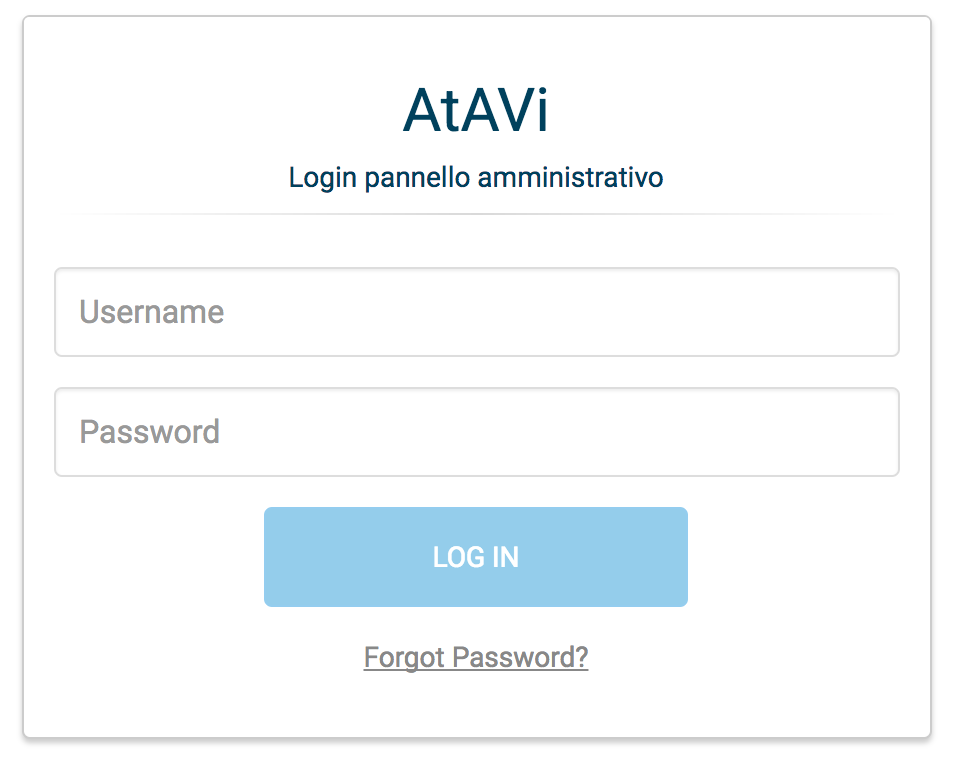
\includegraphics[scale=0.2]{Screenshot/admin-login.png}
		\caption{Pagina di Login}
	\end{figure}
	\textbf{link}: \url{http://localhost:4200/login}
	\newline
	\newline
	Questa pagina permette di accedere a tutte le funzionalità messe a disposizione dal nostro sistema nell'area Amministrativa attraverso l'immissione delle credenziali d'accesso corrette da parte di un Admin o SuperAdmin. Le credenziali richieste sono lo username e la password immesse al momento della registrazione da parte un secondo SuperAdmin. Il sistema riconoscerà automaticamente se le credenziali afferiscono ad un SuperAdmin o ad un Admin, disabilitando alcune funzionalità in quest'ultimo caso.
	\newpage
	\subsection{Pannello d'Amministrazione - Admin}
	\textbf{link}: \url{http://localhost:4200/admin}
	\newline
	\newline
	L'Home Page del Pannello Amministrativo presenta all'Admin le seguenti opportunità di utilizzo:
	\begin{itemize}
		\item{Logout};
		\item{Gestione del proprio profilo};
		\item{Visualizzazione aziende};
		\item{Gestione Slack};
		\item{Gestione domande e risposte}.
	\end{itemize}
	
	\subsubsection{Logout}
	La pressione sul bottone "Log out" in qualsiasi delle pagine che compongono l'area amministrativa provoca la disconnessione dell'utente dal sistema ed il successivo reindirizzamento alla pagina di Login.
	
	\subsubsection{Il tuo profilo}
	\begin{figure}[!h]
		\centering
		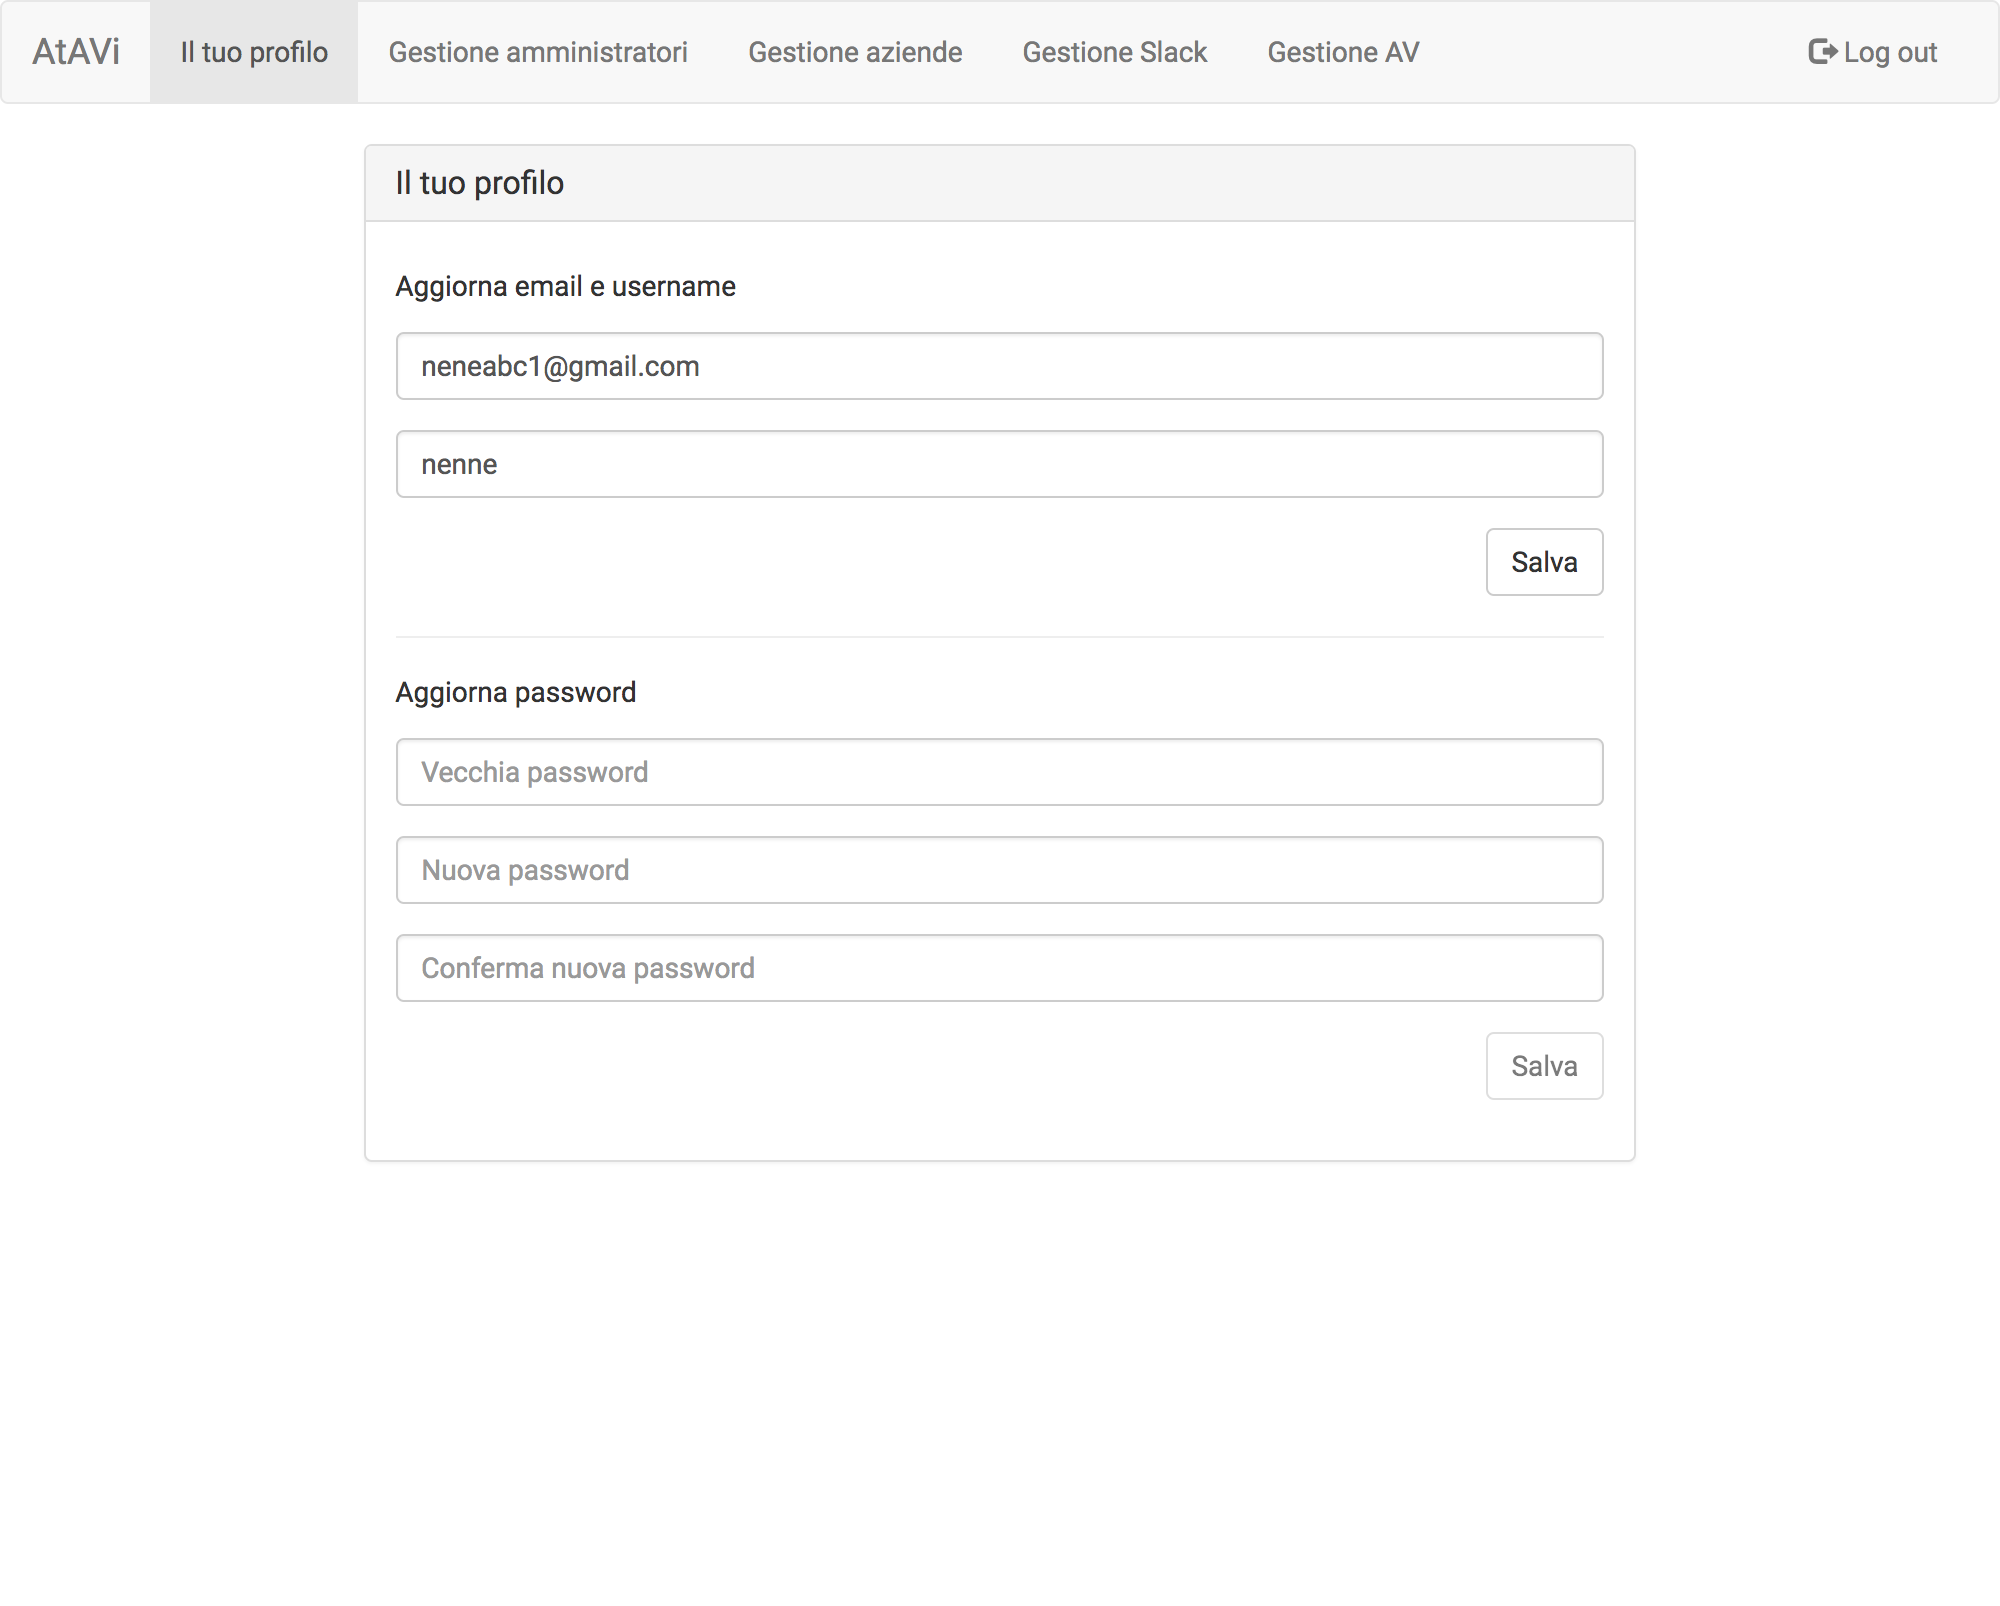
\includegraphics[scale=0.15]{Screenshot/admin-manageProfile.png}
		\caption{Pagina di Gestione del Profilo personale}
	\end{figure}
	Questa pagina permette la visualizzazione dei propri dati personali inseriti all'interno del sistema al momento della registrazione. Di questi dati è resa possibile la modifica delle proprie credenziali di accesso.
	
	\newpage
	\subsubsection{Gestione Aziende}
	\begin{figure}[!h]
		\centering
		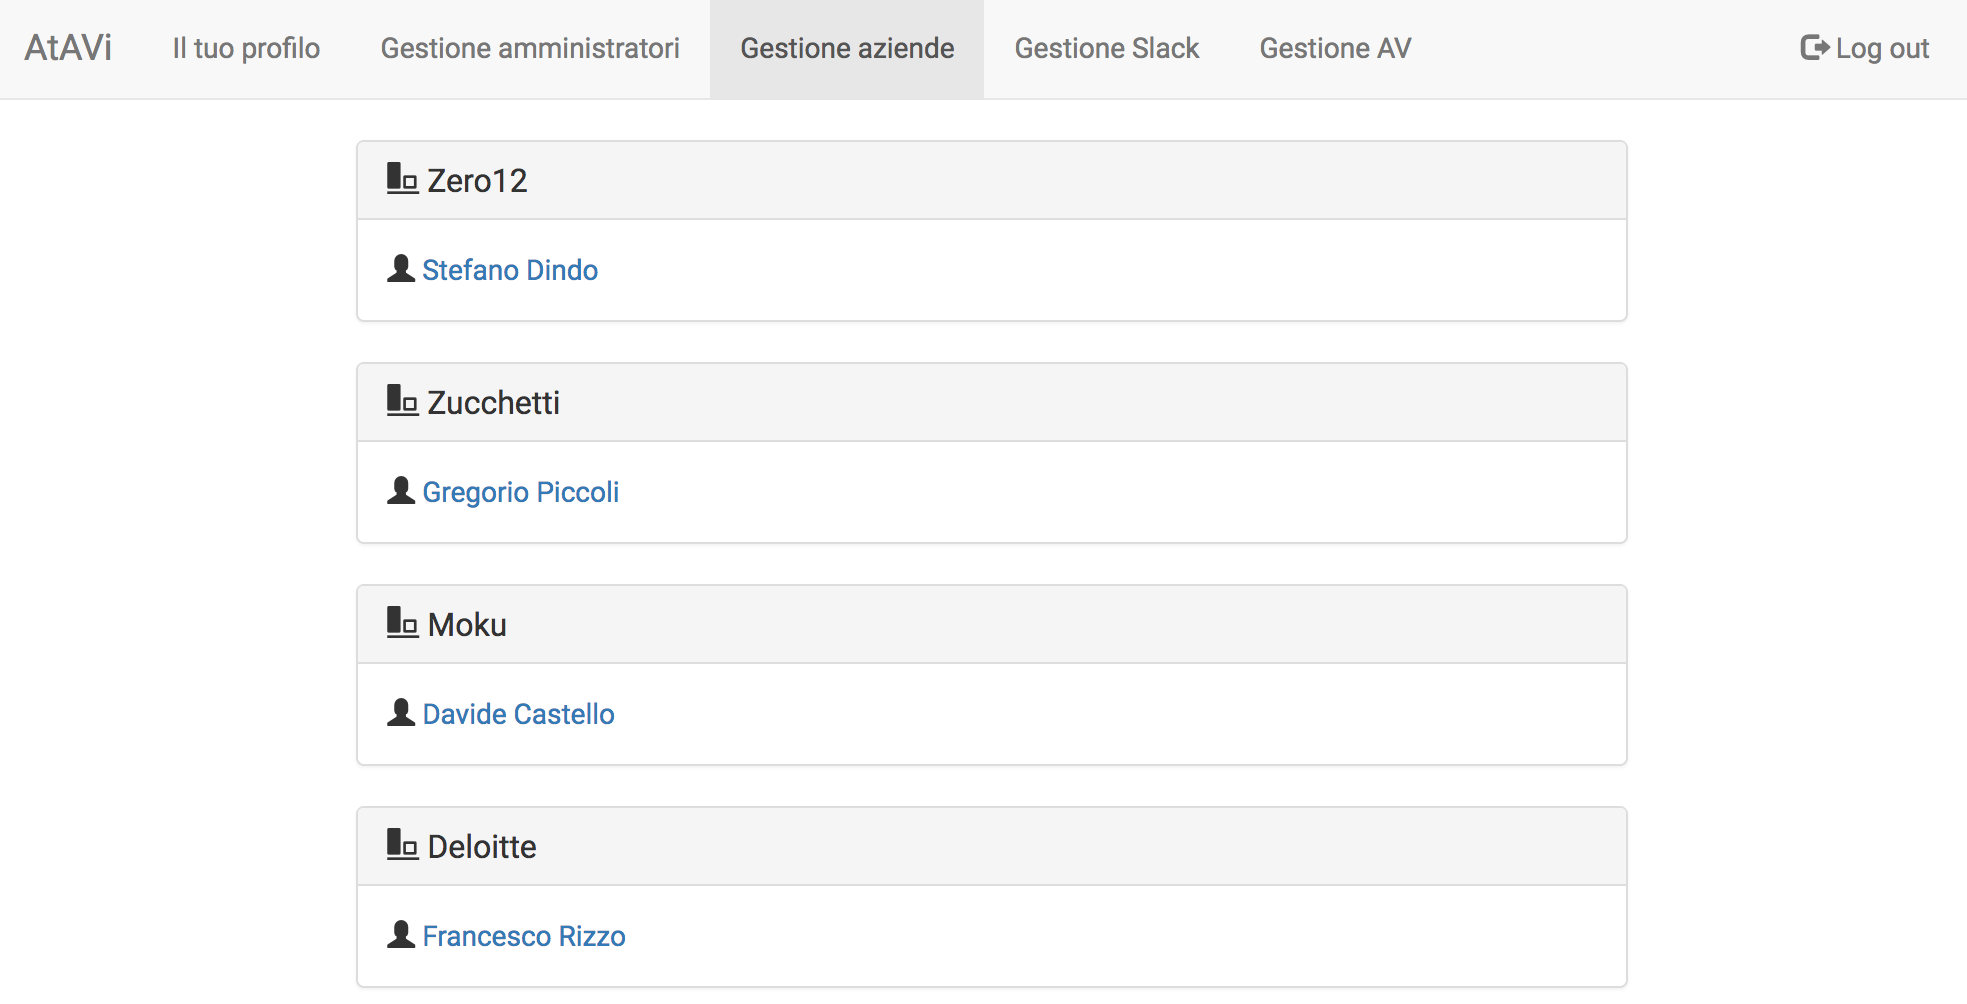
\includegraphics[scale=0.15]{Screenshot/admin-manageFirms.png}
		\caption{Pagina di Gestione delle aziende}
	\end{figure}
	Questa pagina permette di visualizzare tutte le conversazioni fatte dai vari ospiti con l'AV\footnotetext[5]{Assistente Virtuale, in questo caso Alexa di Amazon}. Per visualizzare una conversazione è necessario scegliere l'azienda di cui l'ospite fa parte, il nome di quest'ultimo e la data in cui è avvenuta, dopodiché verrà visualizzata la domanda seguita dalla risposta data.
	
	\newpage
	\subsubsection{Gestione Slack}
	\begin{figure}[!h]
		\centering
		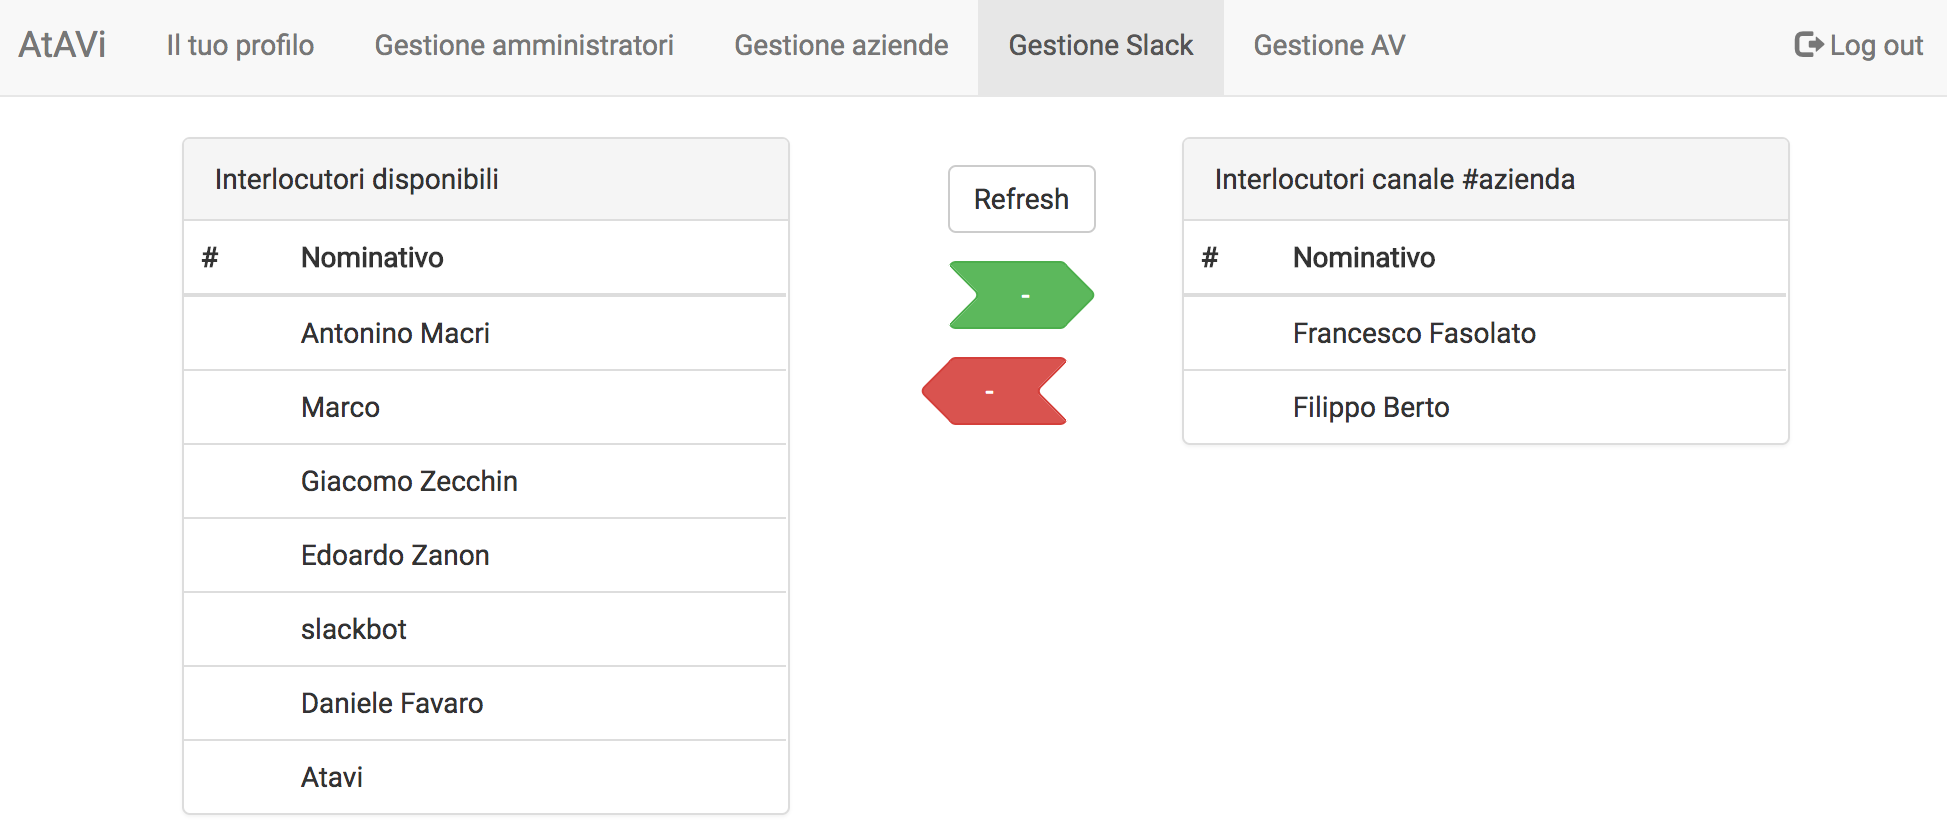
\includegraphics[scale=0.15]{Screenshot/admin-manageSlack.png}
		\caption{Pagina di Gestione degli interlocutori di Slack}
	\end{figure}
	Questa pagina permette di visualizzare la lista di tutti gli interlocutori presenti all'interno del team dell'Azienda creato su Slack e, a fianco di essa, la lista degli interlocutori di default di Slack, ovvero gli interlocutori che vengono inseriti in un canale Slack al momento della sua creazione.
	\newline
	È possibile inoltre aggiungere o togliere degli interlocutori dalla lista di default ed aggiornare il Database tramite l'apposito pulsante di "refresh".
	
	\newpage
	\subsection{Pannello d'Amministrazione - SuperAdmin}
	Oltre alle funzionalità per un normale Admin sovradescritte, un SuperAdmin può accedere anche ad una particolare sezione, realizzata appositamente per la gestione degli Admin.
	\subsubsection{Lista Amministratori}
	\begin{figure}[!h]
		\centering
		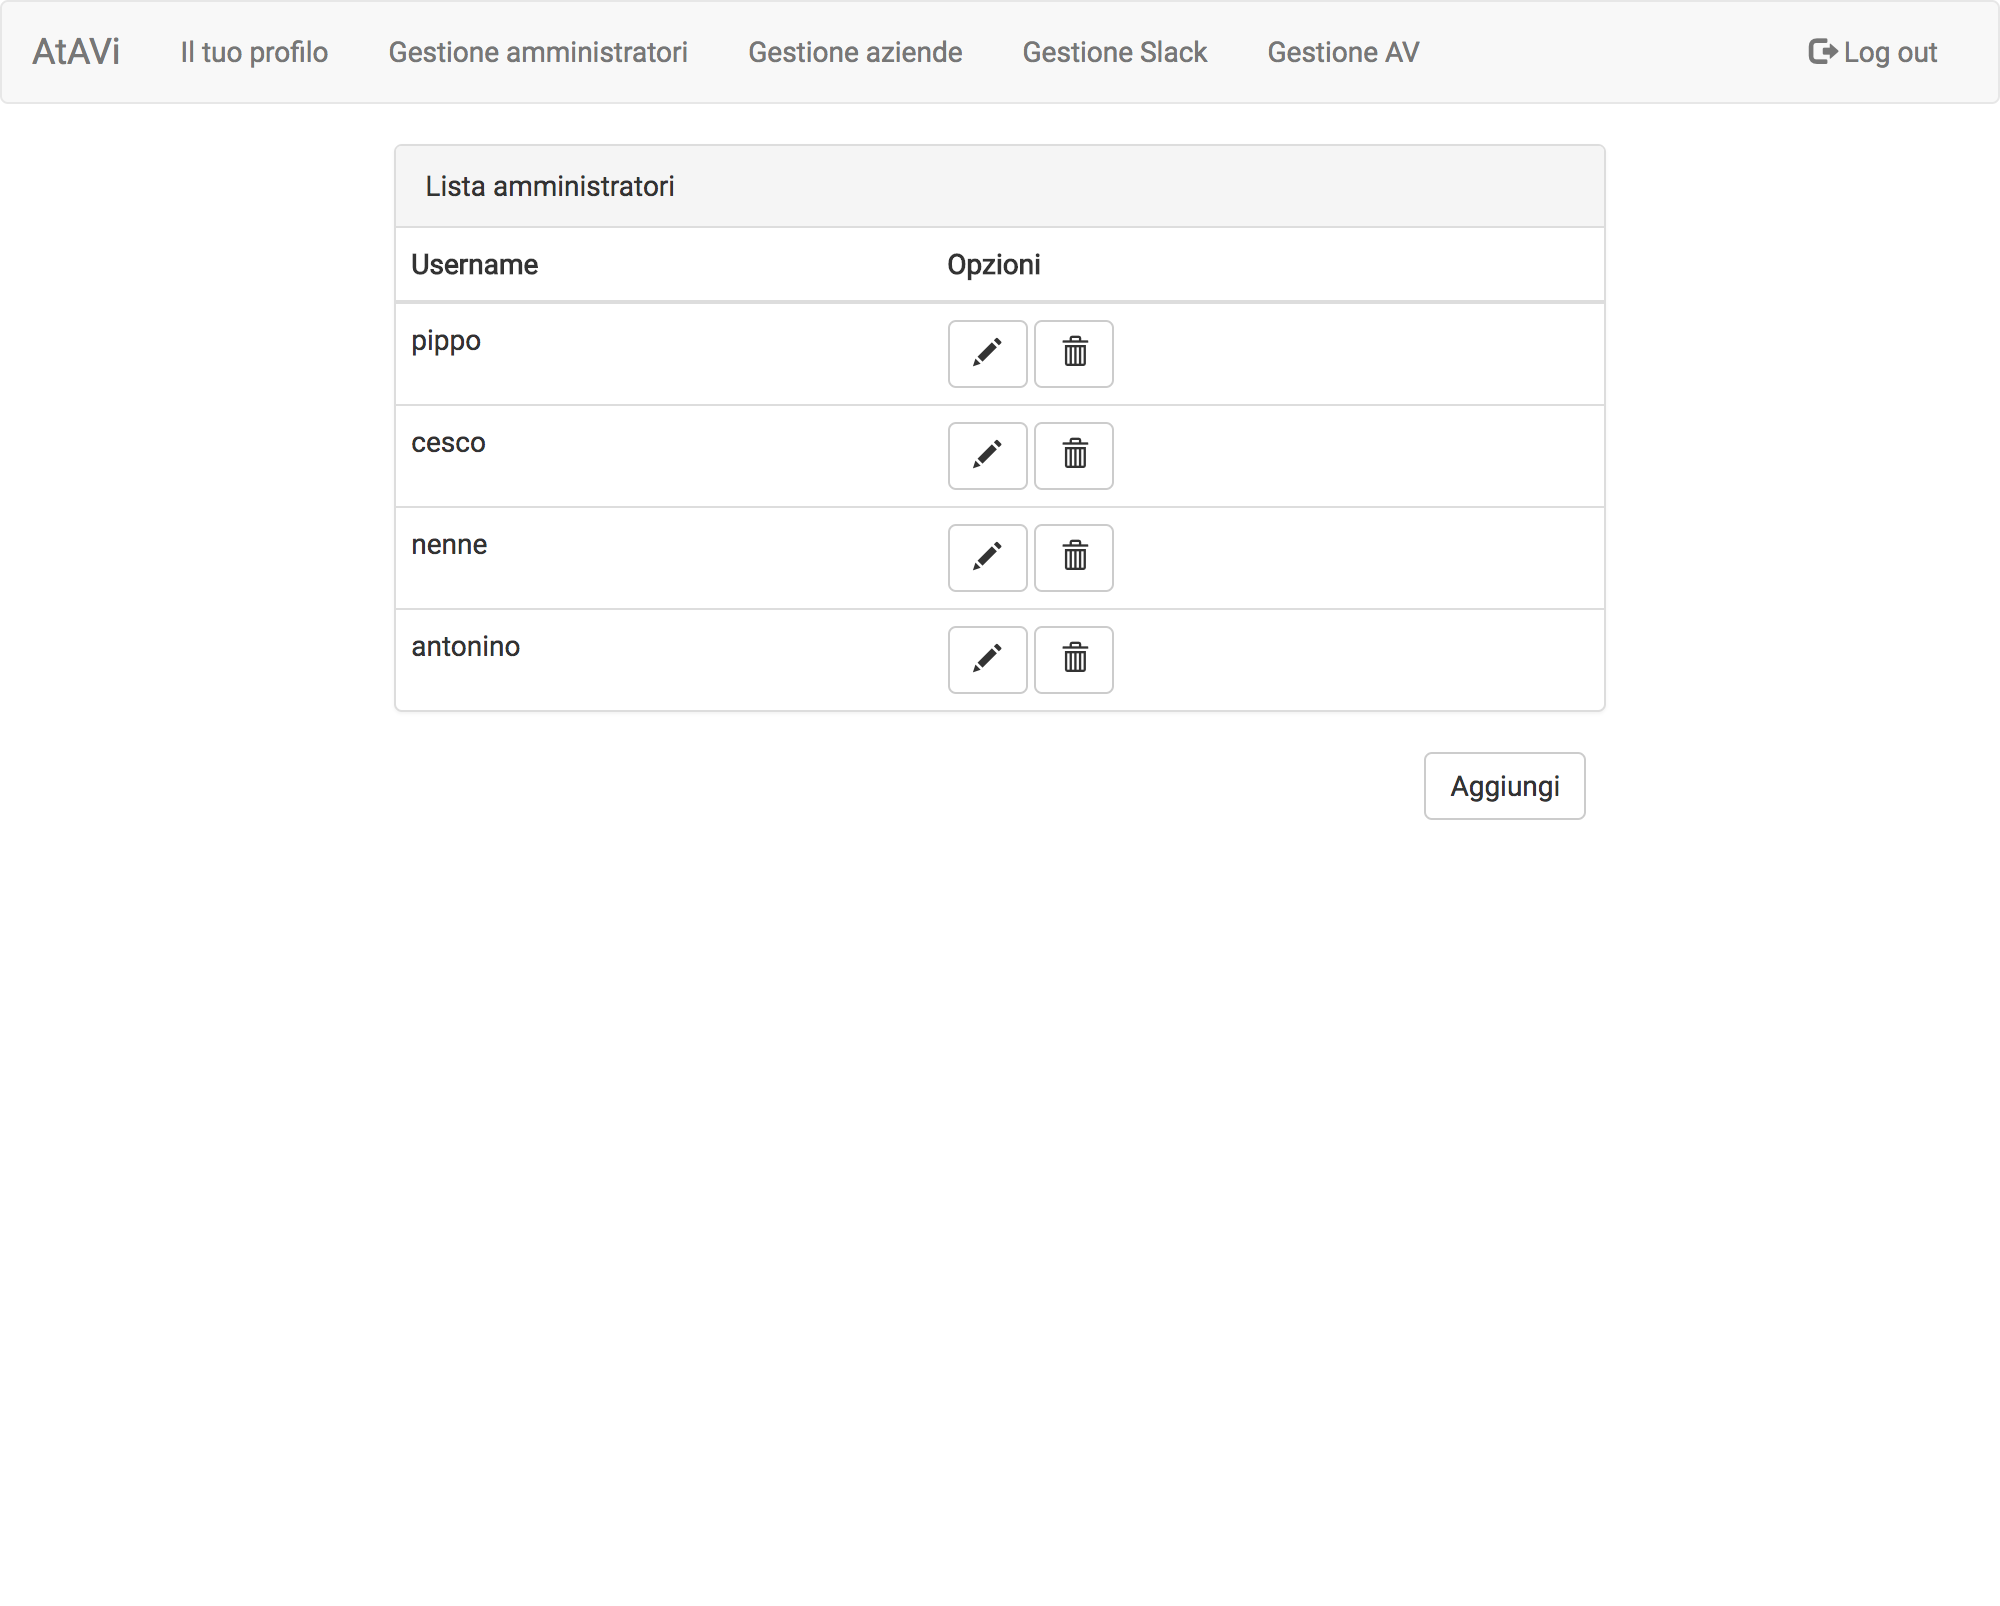
\includegraphics[scale=0.15]{Screenshot/admin-manageAdmins.png}
		\caption{Pagina di Gestione degli Amministratori}
	\end{figure}
	La pagina "Lista Amministratori" mostra a video la lista completa degli amministratori. Selezionando uno degli Admin presenti all'interno di questa lista, un SuperAdmin può entrare nella visualizzazione del profilo dello specifico amministratore ed apportare le seguenti modifiche ai suoi dati:
	\begin{itemize}
		\item{Campo Email};
		\item{Campo Password}.
	\end{itemize}

\end{document}